\documentclass[12pt,a4paper]{article}

\usepackage[utf8]{inputenc}
\usepackage[T1]{fontenc}
\usepackage[english]{babel}
\usepackage{indentfirst}
\usepackage[left=2cm,right=2cm,top=2cm,bottom=2cm]{geometry}
\usepackage{graphicx}

\title{\Large Documentation of the Game \textbf{"Art of Magic"}}
\author{}
\date{}

\begin{document}

\maketitle

\section{Introduction}
\textit{Art of Magic} is a unique strategic card game where players are judged after each battle, evaluating their performance in the duel. The assessment is based on various aspects of their play, including remaining health after the battle, the number of cards of a certain class used, and other key moments of strategy and tactics. Judges analyze these factors to deliver a verdict that can influence future games and strategies of the participants.

\section{Basic Rules}
\subsection{Beginning of the Game}
Players choose their decks of 30 cards and start with 30 health points. The game's goal is to use the cards to reduce the opponent's health to zero.

\subsection{Gameplay}
On their turn, a player draws a card from the deck and can use mana to play cards. Players aim to attack the opponent and defend themselves, using creature cards, spells, and artifacts.

\subsection{Victory}
The player who first reduces the opponent's health to zero wins.

\section{Game Modes}
\subsection{Single Player}
Players can play against computer intelligence.

\subsection{Multiplayer}
Allows players to battle each other online.

\section{Decks and Cards}
\subsection{Deck Creation}
Players create decks by choosing cards from a common pool. Striving for deck balance is crucial.

\subsection{Types of Cards}
\begin{itemize}
    \item Creatures: Can attack and defend.
    \item Spells: Provide various effects.
    \item Artifacts: Offer unique advantages or change the rules.
\end{itemize}

\section{Game Interface}
\textit{Art of Magic} is designed with a user-friendly and intuitive interface, allowing easy management of cards and monitoring of the game's progress.

\section{Conclusion}
\textit{Art of Magic} offers a deep and engaging gameplay experience, combining elements of strategy and tactics. Create your deck and participate in magical duels to claim the title of the greatest mage!

\newpage
\section{Class diagram}
\begin{figure}[h]
\centering 
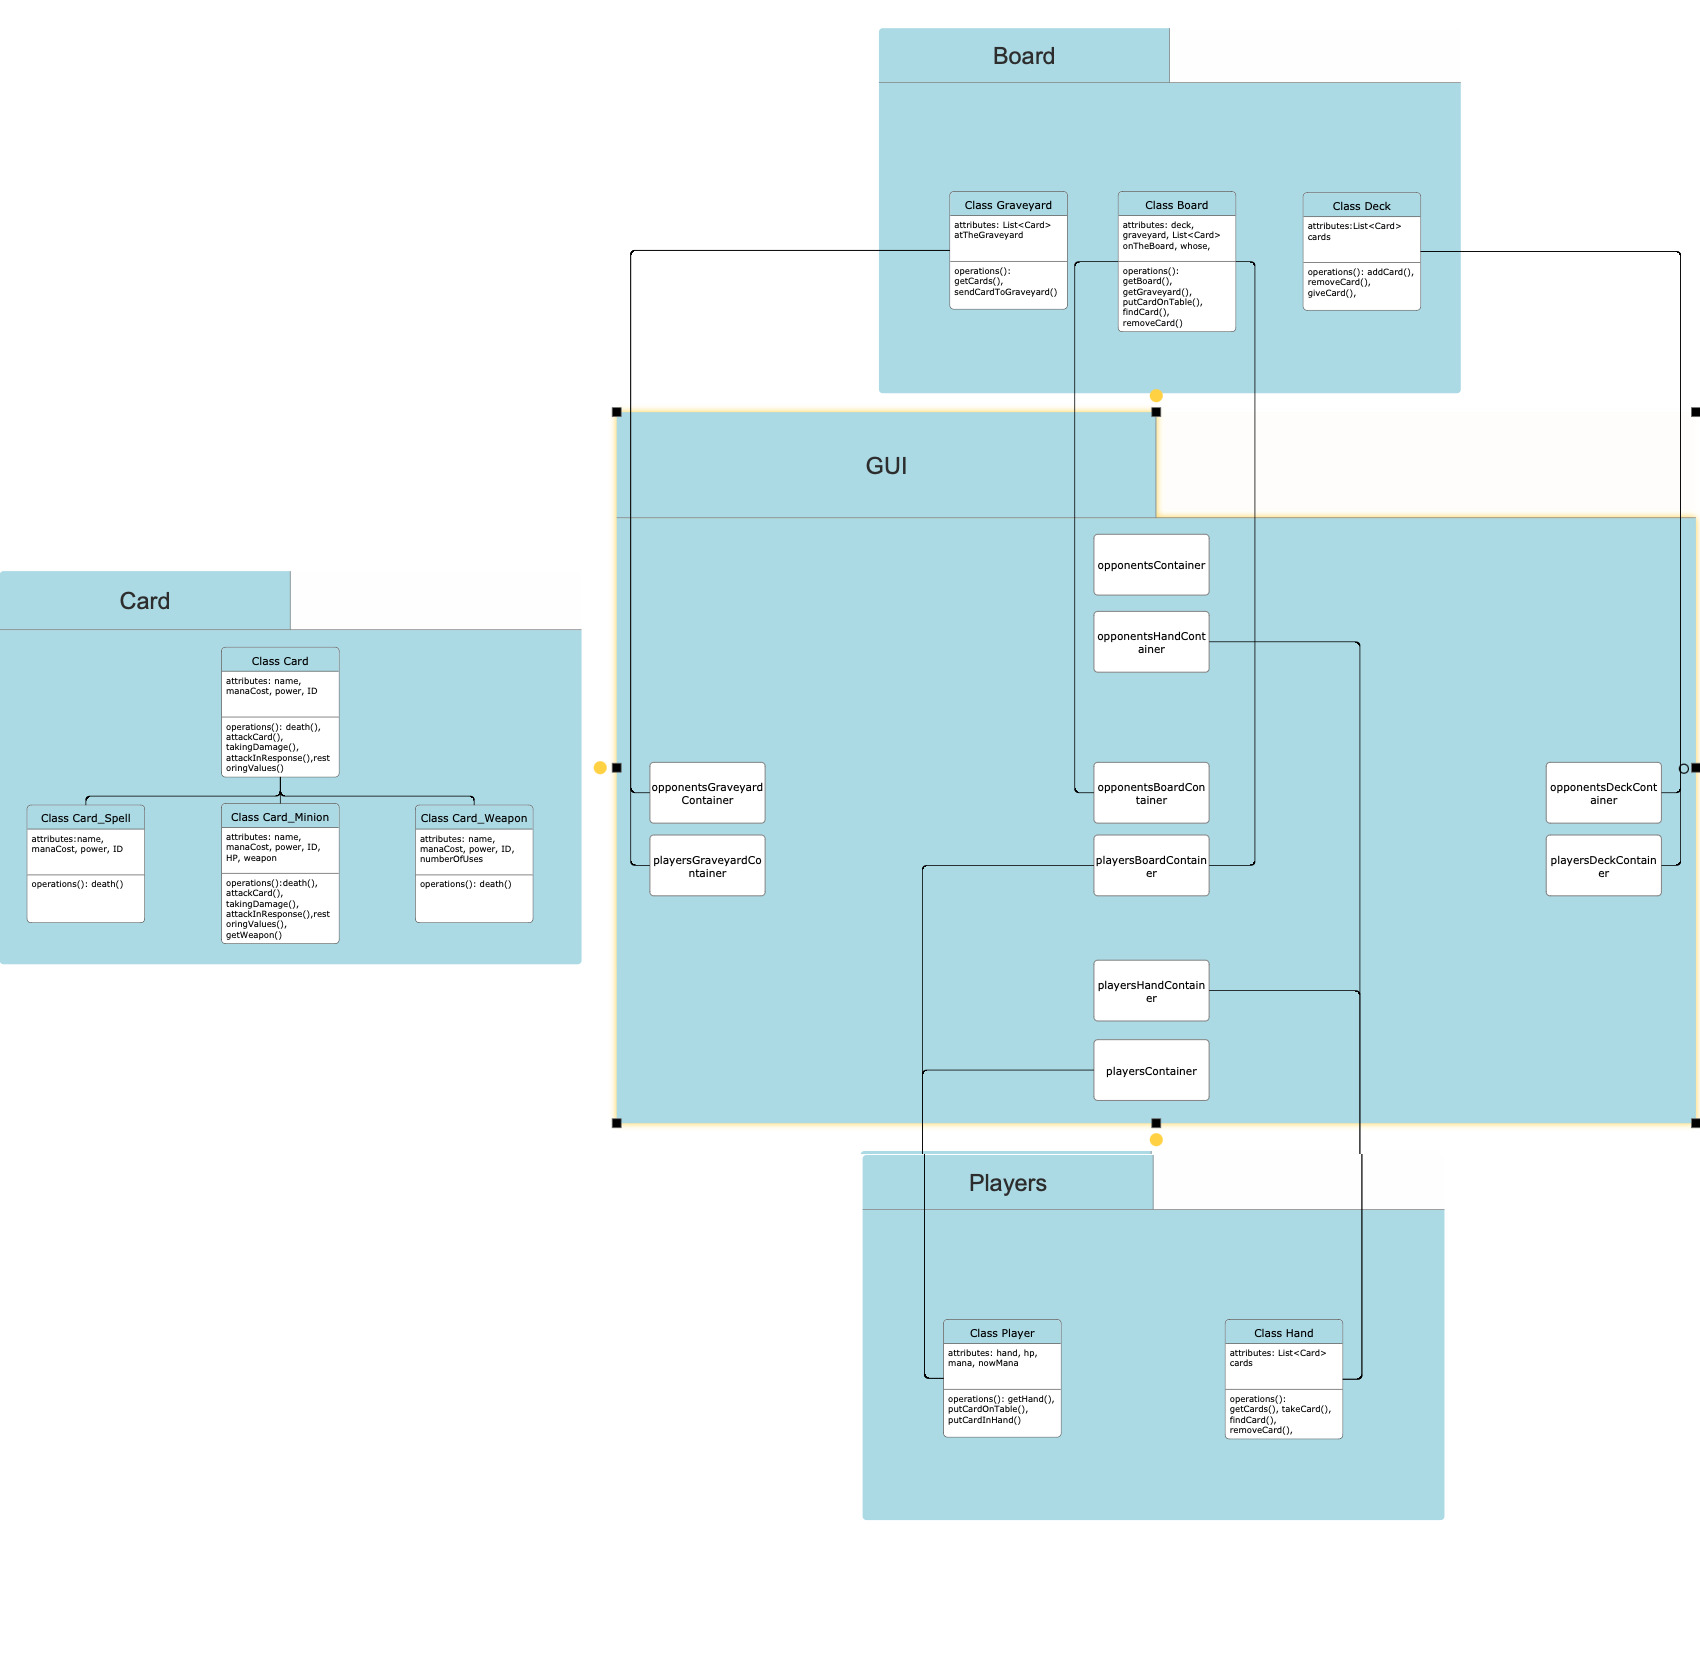
\includegraphics[width=1\textwidth]{img/Diagram.jpg}
\end{figure}


\end{document}
